\chapter{Metodologia}
\label{Cap:MateriaisMetodos}
% Capítulo 3: Materiais e Métodos (ou Metodologia)

\indent
\par A fim de solucionar o problema identificado, foram definidos métodos e estratégias com o objetivo de criar um fluxo de trabalho. A figura \ref{DiagramaDeBlocosIcones} fornece um diagrama ilustrativo e simplificado da solução proposta.

\begin{figure}[H]
    \centering
    \caption{Ilustração da solução}
    
\includegraphics[width=1.0\linewidth]{Imagens/DiagramaDeBlocosIcones.png}
    \caption*{Fonte: Arquivo dos autores (2020)}
    \label{DiagramaDeBlocosIcones}
\end{figure}

\indent
\par Primeiramente alguns dados dos ônibus como, por exemplo, velocidade, tempo de parada, linhas, posição dos veículos são coletados juntamente com imagens do interior dos veículos, que passam por um algoritmo de reconhecimento para identificar a lotação dos mesmos. Paralelamente, informações obtidas por meio de APIs externas enriquecem o conjunto de dados, que por sua vez passa por um tratamento e um treinamento. Após esse processo algumas informações são direcionadas diretamente para o painel de controle enquanto outras passam pela inteligencia artificial para depois serem colocadas no \textit{dashboard}.

\section{Aquisição de dados externos por meio de tarefas}
\indent
\par No que diz respeito à aquisição de dados para alimentação do \textit{dashboard} e sucessiva análise, foi utilizada como principal fonte, a API pública da SP-Trans, mais especificamente os \textit{endpoints} \cite{Schultz2020} “Parada”, “Posicao” e “KMZ”. Cada \textit{endpoint} é responsável por trazer informações como as paradas dos corredores dos ônibus de São Paulo, a posição dos veículos, assim como sua respectiva linha e frota em um dado instante e um arquivo \cite{TechTudo2016} contendo informações de velocidade das linhas, respectivamente.
\indent
\par Vale ressaltar que para a aquisição dos dados do arquivo KMZ, foi realizada uma quebra do arquivo, que originalmente possui as informações em formato XML \cite{Magalhaes2020}. Esse procedimento foi necessário para obter todas as informações já tratadas do arquivo em formato JSON \cite{JSON} para carga do banco de dados.
\indent
\par Adicionalmente a API da SP-Trans, são coletados dados de outras fontes, como Climatempo, Direto dos Trens e \textit{Tickets for Fun}, que são responsáveis por dados como condições meteorológicas, situação das linhas de trens e metrôs em tempo real e localização e data de eventos, respectivamente.
\indent
\par Tendo em vista que todos os dados são coletados com informações em tempo real, é necessário que eles sejam armazenados para que se construa um histórico a fim de se analisar os dados futuramente. Com esse objetivo, foi utilizado o Celery \cite{Celery}, um módulo Python que permite a criação de tarefas assíncronas e agendadas. Tais tarefas foram modeladas para coletar as informações das fontes mencionadas anteriormente em um determinado período de tempo de forma assíncrona e salvá-las em um banco de dados PostgreSQL \cite{PostgreSQL}, criado exclusivamente para o projeto.
\indent
\par Paralelamente à utilização do Celery, foi utilizado um serviço da AWS \cite{AWS}, o \textit{Amazon Simple Queue Service} (SQS), que recebe as tarefas agendadas do Celery e as administra em uma fila, enviando novamente para execução quando for a hora certa. Dessa maneira, as informações em tempo real passaram a ser extraídas ciclicamente por meio das tarefas e salvas em um banco de dados dedicado, gerando um histórico para análise.

\section{Criação de gráficos com Django}
\indent
\par Para a criação do \textit{dashboard} do projeto que exibe informações extraídas a partir dos dados disponíveis no banco de dados, foi utilizado o Django \cite{Django}, um \textit{framework} Python de desenvolvimento rápido para \textit{web}.
\indent
\par O Django utiliza o padrão \textit{model-template-view}, que fornece todas as ferramentas necessárias para o desenvolvimento \textit{web}, desde a criação de um modelo associado ao banco de dados, até o processamento de requisições e criação de páginas \textit{web} dinâmicas de forma robusta e simples. Um de seus principais diferenciais é a padronização dos aplicativos e portabilidade dos mesmos para outros projetos. Isso possibilita uma fácil implementação de módulos e aplicativos externos.
\indent
\par Assim sendo, um dos principais aplicativos utilizados nesse projeto foi o \textit{django-plotly-dash}, que possibilita uma fácil criação de gráficos e painéis que são atualizados em tempo real utilizando apenas código Python, sem a necessidade de escrever código HTML, CSS ou Javascript. Isso possibilitou uma integração direta dos modelos criados no Django com os gráficos. A figura \ref{printDashboard} mostra alguns exemplos de gráficos desenvolvidos com o \textit{django-plotly-dash} para o projeto.

\begin{figure}[H]
    \centering
    \caption{Gráficos criados pelo django-plotly-dash}
    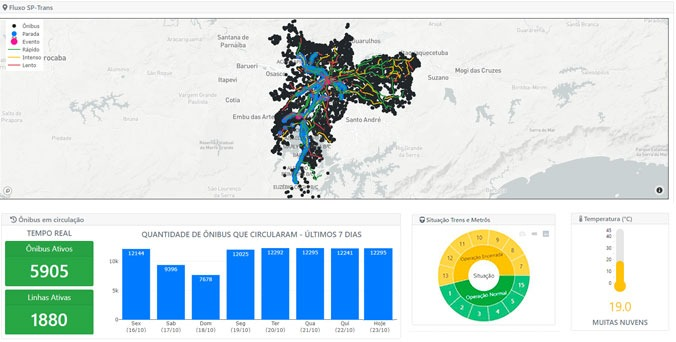
\includegraphics[width=1.0\linewidth]{Imagens/printDashboard.jpeg}
    \caption*{Fonte: Arquivo dos autores (2020)}
    \label{printDashboard}
\end{figure}
\indent
\par Quanto aos modelos mencionados anteriormente, foi criado um modelo para cada informação extraída das APIs externas, estando eles associados à posição dos ônibus, velocidade das vias, linhas e paradas de ônibus, informações das linhas de trens e metrôs, informações meteorológicas e eventos. Todos os modelos estão associados a um banco de dados PostgreSQL, que por possuir uma melhor integração com Python e Django, além de se tratar de um banco de dados relacional e rápido, foi a opção escolhida para o projeto.

\section{APIs com Django REST \textit{Framework}}
\indent
\par O Django REST \textit{Framework} é uma biblioteca para o \textit{Framework} Django que disponibiliza funcionalidades para implementar APIs REST de forma extremamente rápida e fácil. É extremamente simples configurar e criar rotas que aceitam todos os verbos HTTP se comunicando diretamente com o banco de dados e atendendo ao CRUD (\textit{Create} (Criação), \textit{Read} (Consulta), \textit{Update} (Atualização) e \textit{Delete} (Destruição)) \cite{Estevao2016}.
\indent
\par Outra grande vantagem, além da facilidade de implementação, é a criação automática de uma plataforma \textit{web} que centraliza todas as possibilidades de requisições de todas as rotas disponíveis. Nela é possível escolher a forma que deseja visualizar os dados, seja como JSON ou XML o tipo de retorno.
\indent
\par Com as API’s implementadas, é possível acessar os dados da aplicação de forma independente do \textit{dashboard}. Assim, outras pessoas podem ter acesso a esses dados para novas e futuras análises. Alguns dos \textit{endpoints} criados disponibilizam dados como de velocidade, posição, linhas, paradas, metrô, trem e clima.

\begin{figure}[H]
    \centering
    \caption{Rotas das APIs dentro da plataforma \textit{web} disponibilizada pelo Django}
    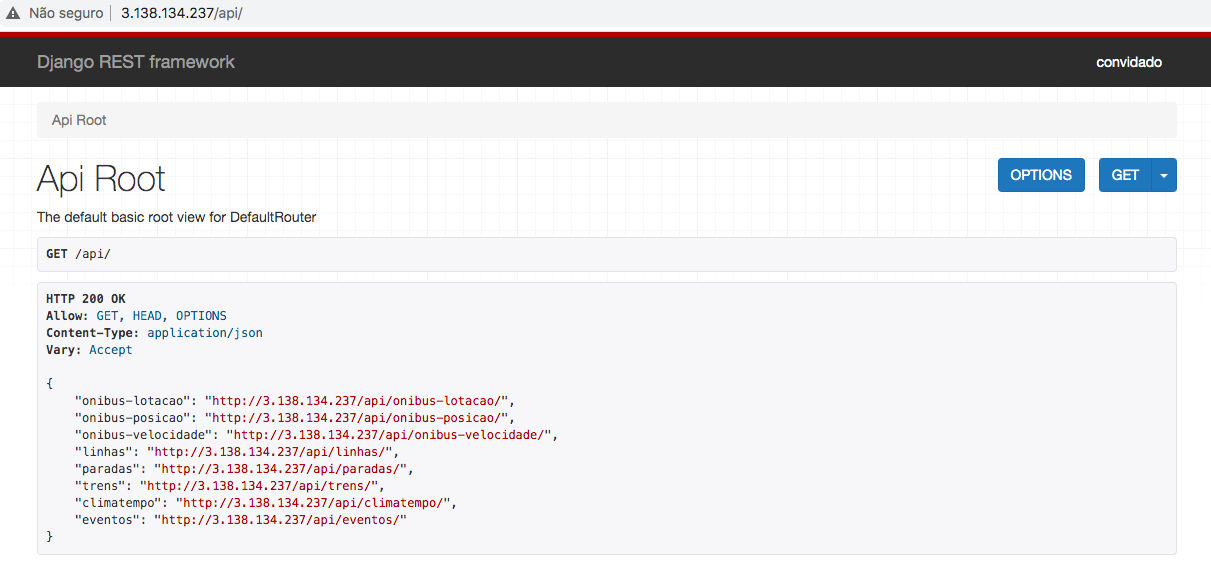
\includegraphics[width=1.0\linewidth]{Imagens/rotasDisponiveis.png}
    \caption*{Fonte: Arquivo dos autores (2020)}
    \label{rotasDisponiveis}
\end{figure}

\begin{figure}[H]
    \centering
    \caption{Exemplo de retorno JSON do \textit{endpoint} /api/onibus-lotacao}
    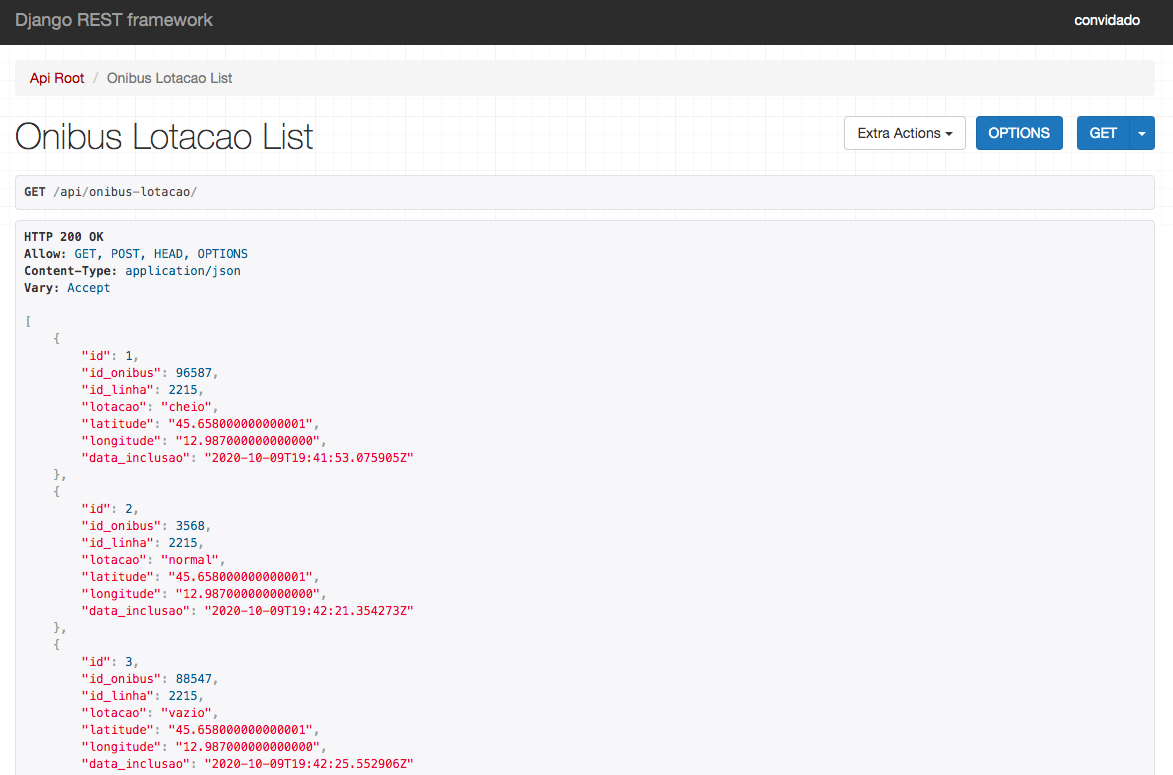
\includegraphics[width=1.0\linewidth]{Imagens/onibusLotacaoExemplo.png}
    \caption*{Fonte: Arquivo dos autores (2020)}
    \label{onibusLotacaoExemplo}
\end{figure}
\indent
\par Na figura \ref{rotasDisponiveis}, podemos visualizar uma lista com todas as rotas disponíveis. Um exemplo de requisição nessas rotas pode ser visualizado na imagem \ref{onibusLotacaoExemplo}, onde é realizada uma requisição do tipo \textit{GET} no \textit{endpoint} ‘onibus-lotacao’. 
\indent
\par Podemos ver que a resposta foi do tipo JSON, retornando todas as informações disponíveis como, id, id\_onibus, id\_linha, lotação, latitude, longitude, data\_inclusao.

\section{\textit{Endpoints}}
\indent
\par Na imagem \ref{rotasDisponiveis}, podemos visualizar todos os \textit{endpoints} disponíveis, cada um deles possui suas informações e funções. No apêndice \ref{app:apendiceA}, uma breve descrição de cada uma delas, e como utilizá-las com os verbos \textit{GET} e \textit{POST}, assim como uma prévia do retorno das informações.
\indent
\par Foi escolhido apresentar as requisições \textit{GET} e \textit{POST} pois são através delas que o \textit{dashboard} consome os dados e que as APIs externas salvam as informações dentro do nosso banco de dados.

\section{Infraestrutura de nuvem}
\indent
\par Pela necessidade de estar disponível a qualquer momento e de capturar o máximo de informação possível, decidimos disponibilizar o nosso sistema na nuvem, utilizando a plataforma da Amazon, principalmente os recursos da \textit{Elastic Cloud Compute} (EC2). A nossa infraestrutura gira em torno de uma máquina Linux, da categoria t2.medium, que se provou o mínimo necessário para executar o nosso sistema e aguentar a carga de algumas visitas simultâneas.
\indent
\par Começando pela máquina, as instâncias EC2 t2.medium são máquinas com 2 núcleos dedicados, 4GB de memória RAM, indicadas tanto para o uso como plataforma de desenvolvimento quanto para servidores \textit{web}. Entre suas características temos processadores com um \textit{clock} relativamente alto e ao mesmo tempo um custo baixo em comparação com as outras soluções oferecidas pela Amazon, como instâncias t3 ou A1. 
\indent
\par Decidimos usar a instância t2.medium após realizar testes tanto com a t2.micro, que é gratuita para as 750 primeiras horas por mês, quanto a t2.small, que é totalmente paga, mas mais econômica que a t2.medium. A modalidade micro apresentou dificuldades logo nos primeiros instantes, apesar de ser capaz de executar o \textit{dashboard} em Django paralelo ao banco de dados PostgreSQL, quando começamos a rodar as tasks do Celery para captura de dados, o processamento disponível para ela não foi o suficiente, atingindo 100\% de uso do núcleo disponível e deixando o sistema inutilizável, mesmo com uma única pessoa acessando. Já a instância t2.small se mostrou capaz de executar as \textit{tasks} simultaneamente ao \textit{dashboard} e o banco de dados, porém ao começar a receber acessos no \textit{dashboard} o sistema não conseguia dar conta das requisições e apresentava uma constante lentidão. 
\indent
\par Com isso, chegamos a conclusão que a instância mínima para rodarmos o nosso projeto com segurança é a t3.medium, e mesmo assim rapidamente consumimos todo o seu armazenamento em pouco menos de uma semana, após isso expandimos ele de 7GB para 50GB, o que nos daria uma margem de segurança até a conclusão do projeto. Apesar da instância média ser o suficiente para o nosso uso durante o desenvolvimento, notamos que a sua configuração não seria o suficiente para um momento de fluxo constante no sistema por conta do uso do processador, que se aproxima de 100\% sempre que tem mais de dois navegadores acessando simultaneamente, por isso durante o Eureka, decidimos usar a instância t2.2xlarge, com 8 vCores e 32GB de memória ram, o que se mostrou suficiente para momentos com cerca de 10 acessos simultâneos.

\par Para o acesso à instância pelo navegador, usamos uma implantação simples do NGINX \cite{NGINX}, um servidor web muito popular por sua facilidade de uso e segurança. O servidor é o primeiro lugar que as requisições web chegam na instância e o NGINX distribui essas requisições para cada local definido em suas configurações, na nossa situação temos uma rota só para os arquivos estáticos e outra para o sistema em si. Isso permite uma velocidade de resposta maior que se todos os elementos estivessem na mesma e rota e facilita a manutenção dos arquivos do sistema.




